\documentclass[a4paper,12pt]{article}
\usepackage[utf8]{inputenc}
\usepackage[T1]{fontenc}
\usepackage{amsmath, amssymb}
\usepackage{graphicx}
\usepackage{geometry}
\geometry{margin=1in}
\usepackage{hyperref}
\usepackage{float}
\usepackage{caption}
\usepackage{enumitem}
\usepackage{listings}
\usepackage{xcolor}
\usepackage{titling}
\usepackage{times}

% Beginning the document
\begin{document}

% Creating the title page
\title{Arbitrary Precision Arithmetic Library: Project Report \\ Software Development Fundamentals (CS1023)}
\author{Shiva Ganesh Adepu \\ ID: CS24BTECH11003}
\date{May 2025}
\maketitle

% Adding a table of contents
\tableofcontents
\newpage

% Introducing the project and its objectives
\section{Introduction}
This report outlines the development of an arbitrary precision arithmetic library in Java, The library, implemented in the \texttt{arbitraryarithmetic} package, supports infinite-precision arithmetic operations for both integers and floating-point numbers through two classes: \texttt{AInteger} and \texttt{AFloat}. The project also includes a command-line interface via the \texttt{MyInfArith} class and a Python script for compilation and execution.

The library supports addition, subtraction, multiplication, and division operations without round-off errors, adhering to the project requirement of preserving complete numerical information. Decimal precision for floating-point operations is truncated at 30 digits, following Java's \texttt{BigDecimal} class behavior.

% Describing the design decisions and referencing the UML diagram
\section{Design}
The library is structured around two core classes within the \texttt{arbitraryarithmetic} package: \texttt{AInteger} for integer arithmetic and \texttt{AFloat} for floating-point arithmetic. Key design decisions include:

\begin{itemize}
    \item \textbf{String-based Representation}: Both classes internally represent numbers as strings to handle arbitrary precision, avoiding limitations of Java's primitive types.
    \item \textbf{Sign Handling}: The \texttt{AInteger} class uses a boolean \texttt{isPositive} to track the sign, while \texttt{AFloat} relies on \texttt{AInteger} for sign management.
    \item \textbf{Decimal Tracking in AFloat}: The \texttt{AFloat} class tracks decimal places using \texttt{NumOfDigitsAfterDecimal}, enabling precise floating-point operations.
    \item \textbf{Operator Overloading Simulation}: Since Java does not support operator overloading, methods like \texttt{add}, \texttt{subtract}, \texttt{multiply}, and \texttt{divide} are implemented to simulate operator behavior.
    \item \textbf{Reusability}: Helper methods like \texttt{removeLeadingZeros} and \texttt{compareStrings} in \texttt{AInteger} are reused across operations to ensure consistency.
\end{itemize}

\newpage
The class structure and relationships are illustrated in the UML diagram (see Figure~\ref{fig:uml}).

% Including a placeholder for the UML diagram
\begin{figure}[H]
    \centering
    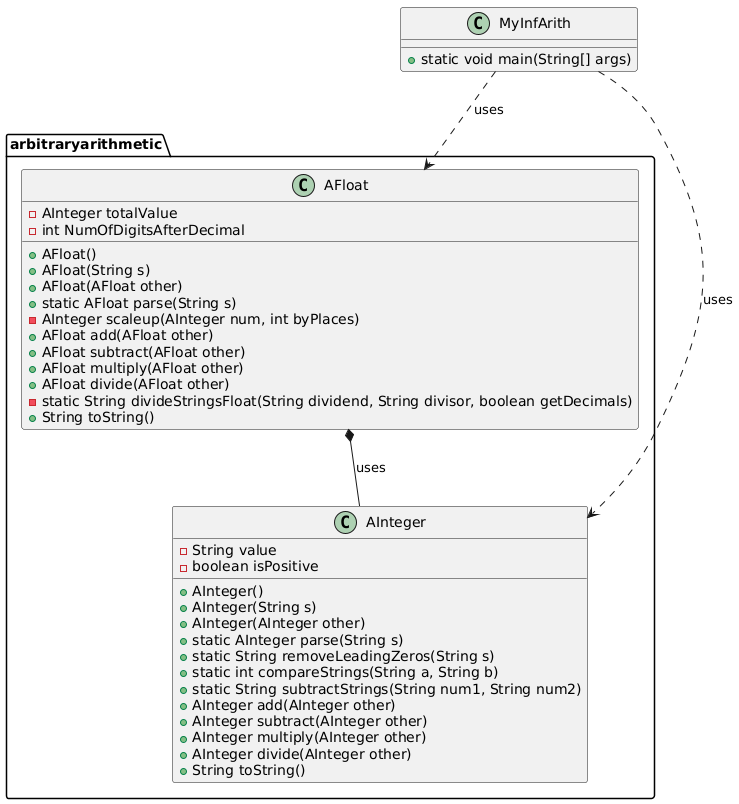
\includegraphics[width=0.8\textwidth]{uml.png} % Placeholder for UML diagram
    \caption{UML Class Diagram for the Arbitrary Precision Arithmetic Library}
    \label{fig:uml}
\end{figure}

\section{Logic of Classes}
This section details the core logic behind the \texttt{AInteger} and \texttt{AFloat} classes, focusing on how they handle arbitrary precision arithmetic and the role of method overriding.

\subsection{AInteger Class Logic}
The \texttt{AInteger} class is designed to handle arbitrary precision integer arithmetic. Numbers are stored as strings in the \texttt{value} field, with a boolean \texttt{isPositive} to track the sign. The core logic revolves around string manipulation to perform arithmetic operations:

\begin{itemize}
    \item \textbf{Constructor and Parsing}: The class provides constructors to initialize an \texttt{AInteger} from a string or another \texttt{AInteger}. The \texttt{parse} method converts a string input into an \texttt{AInteger}, handling signs and leading zeros using \texttt{removeLeadingZeros}.
    \item \textbf{Arithmetic Operations}: Methods like \texttt{add}, \texttt{subtract}, \texttt{multiply}, and \texttt{divide} implement arithmetic by manipulating digit strings. For example, \texttt{addStrings} and \texttt{subtractStrings} perform digit-by-digit addition and subtraction, managing carries and borrows, while \texttt{multiplyStrings} and \texttt{divideStrings} use schoolbook algorithms for multiplication and division.
    \item \textbf{Utility Methods}: Helper methods like \texttt{compareStrings} compare two number strings by length and digit values, ensuring correct ordering for subtraction and division.
    \item \textbf{Method Overriding}: The \texttt{toString} method is overridden (using Java's \texttt{@Override} annotation) to provide a string representation of the number, ensuring the sign is correctly displayed (e.g., adding a negative sign if \texttt{isPositive} is \texttt{false}).
\end{itemize}

The \texttt{@Override} annotation in \texttt{toString} indicates that the method overrides the default \texttt{toString} implementation from Java's \texttt{Object} class, ensuring proper string conversion for \texttt{AInteger} objects.

\subsubsection{Arithmetic Operations Logic}
The following details the logic for each arithmetic operation in \texttt{AInteger}:

\begin{itemize}
    \item \textbf{Addition}: The \texttt{add} method first checks the signs of the operands. If both are positive or both negative, it calls \texttt{addStrings} to perform digit-by-digit addition, handling carries (e.g., for "123" + "456", it computes each column: 3+6=9, 2+5=7, 1+4=5, resulting in "579"). If signs differ, it converts addition into subtraction by comparing magnitudes with \texttt{compareStrings} and calling \texttt{subtractStrings}.
    \item \textbf{Subtraction}: The \texttt{subtract} method also considers signs. If both operands have the same sign, it uses \texttt{subtractStrings} for digit-by-digit subtraction with borrowing (e.g., "456" - "123" computes 6-3=3, 5-2=3, 4-1=3, yielding "333"). If signs differ, it converts subtraction into addition. The \texttt{compareStrings} method ensures the larger number is subtracted from the smaller one, adjusting the sign of the result.
    \item \textbf{Multiplication}: The \texttt{multiply} method implements a schoolbook multiplication algorithm via \texttt{multiplyStrings}. It multiplies each digit of one number by each digit of the other, tracking carries and summing partial products (e.g., "12" × "13" computes 12×3=36 and 12×1=12, then adds with proper place alignment: 36 + 120 = 156). Signs are handled by setting the result's \texttt{isPositive} based on the XOR of the operands' signs.
    \item \textbf{Division}: The \texttt{divide} method uses \texttt{divideStrings}, implementing long division. It repeatedly subtracts the divisor from the dividend, counting how many times it fits (e.g., "100" ÷ "4" subtracts 4 from 100, 25 times, yielding "25"). It handles division by zero by throwing an exception and sets the sign of the result based on the operands' signs.
\end{itemize}

\subsection{AFloat Class Logic}
The \texttt{AFloat} class extends the functionality of \texttt{AInteger} to support floating-point arithmetic. It reuses much of \texttt{AInteger}'s logic, with additional handling for decimal points:

\begin{itemize}
    \item \textbf{Structure and Reuse}: \texttt{AFloat} stores its value as an \texttt{AInteger} in the \texttt{totalValue} field, with an integer \texttt{NumOfDigitsAfterDecimal} to track the number of digits after the decimal point. This allows \texttt{AFloat} to leverage \texttt{AInteger}'s integer arithmetic logic by converting floating-point numbers into integers (e.g., 12.34 is stored as 1234 with \texttt{NumOfDigitsAfterDecimal = 2}).
    \item \textbf{Decimal Handling}: Arithmetic operations in \texttt{AFloat} first align the decimal points of operands by scaling them (using \texttt{scaleup}), then perform the operation using \texttt{AInteger} methods, and finally adjust the result's decimal position. For example, in \texttt{add}, two \texttt{AFloat} numbers are scaled to have the same number of decimal places, added as \texttt{AInteger}s, and the result is converted back to an \texttt{AFloat}.
    \item \textbf{Division Precision}: The \texttt{divideStringsFloat} method ensures floating-point division results are truncated at 30 decimal places, as per project requirements, while reusing \texttt{AInteger}'s division logic for the core computation.
    \item \textbf{Method Overriding}: Similar to \texttt{AInteger}, \texttt{AFloat} overrides the \texttt{toString} method using the \texttt{@Override} annotation. This method converts the \texttt{totalValue} back into a floating-point string by inserting the decimal point at the correct position based on \texttt{NumOfDigitsAfterDecimal}.
\end{itemize}

The use of \texttt{@Override} in both classes ensures that the \texttt{toString} method adheres to Java's object-oriented principles, providing a customized string representation for each class while maintaining compatibility with the \texttt{Object} superclass.

\subsubsection{Arithmetic Operations Logic}
The following details the logic for each arithmetic operation in \texttt{AFloat}, building on \texttt{AInteger}'s logic:

\begin{itemize}
    \item \textbf{Addition}: The \texttt{add} method aligns the decimal points of the two \texttt{AFloat} numbers by scaling them with \texttt{scaleup} (e.g., for 12.34 + 56.7, it converts to 1234 and 5670 with \texttt{NumOfDigitsAfterDecimal = 2}). It then uses \texttt{AInteger}'s \texttt{add} method to compute the sum (1234 + 5670 = 6904), adjusts the decimal position in the result (69.04), and returns a new \texttt{AFloat}.
    \item \textbf{Subtraction}: The \texttt{subtract} method follows a similar process, aligning decimals (e.g., 56.7 - 12.34 becomes 5670 - 1234), uses \texttt{AInteger}'s \texttt{subtract} (5670 - 1234 = 4436), and adjusts the result's decimal position (44.36). Sign handling is inherited from \texttt{AInteger}.
    \item \textbf{Multiplication}: The \texttt{multiply} method first multiplies the \texttt{totalValue} of both \texttt{AFloat} numbers using \texttt{AInteger}'s \texttt{multiply} (e.g., 12.34 × 56.78 becomes 1234 × 5678 = 7006652). It then calculates the new \texttt{NumOfDigitsAfterDecimal} by adding the decimal places of the operands (2 + 2 = 4), resulting in 700.6652.
    \item \textbf{Division}: The \texttt{divide} method uses \texttt{divideStringsFloat}, which scales the dividend to increase precision (e.g., for 12.34 ÷ 56.78, it scales 1234 to 123400... with 30 extra digits), performs division using \texttt{AInteger}'s logic (yielding a quotient with extra precision), and truncates the result at 30 decimal places (e.g., 0.217330...).
\end{itemize}





% Providing instructions on how to use the library
\section{Usage Instructions}
The library can be used in two modes: as a command-line application or as a reusable library.

\subsection{As a Command-Line Application}
The \texttt{MyInfArith} class provides a command-line interface. It accepts four arguments:
\begin{itemize}
    \item \texttt{<int/float>}: Specifies the type of operation (\texttt{int} for integers, \texttt{float} for floating-point).
    \item \texttt{<add/sub/mul/div>}: Specifies the operation.
    \item \texttt{First operand}: The first number as a string.
    \item \texttt{Second operand}: The second number as a string.
\end{itemize}

Example usage:
\begin{lstlisting}[language=bash]
java MyInfArith int add 23650078224912949497310933240250 42939783262467113798386384401498
\end{lstlisting}
Output:
\begin{lstlisting}
66589861487380063295697317641748
\end{lstlisting}

A Python script (\texttt{PythonScript.py}) is provided to compile and run the project. Run it as follows:
\begin{lstlisting}[language=bash]
python3 PythonScript.py
\end{lstlisting}

\subsection{As a Library}
The \texttt{arithmetic.jar} file in the \texttt{arbitraryarithmetic} directory can be included in other Java projects. Import the classes as follows:
\begin{lstlisting}[language=Java]
import arbitraryarithmetic.AInteger;
import arbitraryarithmetic.AFloat;
\end{lstlisting}

Example usage in code:
\begin{lstlisting}[language=Java]
AInteger a = new AInteger("123456789");
AInteger b = new AInteger("987654321");
AInteger sum = a.add(b);
System.out.println(sum); // Outputs: 1111111110
\end{lstlisting}

% Placeholder for the git commit snapshot


% Discussing the limitations of the library
\section{Limitations}
The library has the following limitations:
\begin{itemize}
    \item \textbf{Performance}: String-based arithmetic operations are slower than native types, especially for large numbers.
    \item \textbf{Decimal Precision}: Floating-point division is capped at 30 decimal places, which may not suffice for applications requiring higher precision.
    \item \textbf{Error Handling}: Division by zero is handled, but other edge cases (e.g., extremely large inputs) may lead to memory issues.
    \item \textbf{Lack of Optimization}: Operations like multiplication and division could be optimized using advanced algorithms (e.g., Karatsuba multiplication).
\end{itemize}

% Outlining the verification approach
\section{Verification Approach}
The library was tested across multiple stages:
\begin{itemize}
    \item \textbf{Unit Testing}: Individual methods in \texttt{AInteger} and \texttt{AFloat} were tested with small inputs (e.g., \texttt{"123"} + \texttt{"456"}).
    \item \textbf{Test Cases}: The provided test cases were executed via \texttt{MyInfArith}, covering integer and floating-point operations (e.g., \texttt{java MyInfArith float div 8792726365283060579833950521677211.0 493835253617089647454998358}).
    \item \textbf{Edge Cases}: Tested with zero, negative numbers, and large inputs to ensure robustness.
\end{itemize}

% Sharing key learnings from the project
\section{Key Learnings}
This project provided valuable insights:
\begin{itemize}
    \item \textbf{Arbitrary Precision}: Implementing arithmetic without round-off errors required careful string manipulation and decimal tracking.
    \item \textbf{Java Limitations}: Working around Java's lack of operator overloading necessitated method-based operation design.
    \item \textbf{Project Management}: Using Git for version control and tagging stages improved collaboration and tracking.
    \item \textbf{Documentation}: Writing detailed comments and a LaTeX report enhanced the project's clarity and usability.
\end{itemize}

% Ending the document
\end{document}